\documentclass[letterpaper]{article}
\usepackage[spanish]{babel}
\usepackage[utf8]{inputenc}
\usepackage{graphicx}
\usepackage{amsmath}

\title{Proyecto de Ingeniería de Software II}
\author{Acuña Yeomans Eduardo\\Contreras Mejía Daniel\\Valle Ruiz Francisco Manuel}
\date{Lunes 2 de Junio del 2014}

\begin{document}

\maketitle

%%%
\section{Presentación}

\subsection{Sobre Sabrosoftware}
Sabrosoftware es la compañía de desarrollo de software con mayor prestigio en la clase de Ingeniería de Software II impartida por el profesor Adrián en la primera mitad del año 2014 en la Licenciatura en Ciencias de la Computación del Departamento de Matemáticas de la Universidad de Sonora. Engendrada en el 2013 como parte de un proyecto de Ingeniería de Software I, Sabrosoftware ha aprendido de sus errores en el previo trabajo y planea posicionarse como la compañía de desarrollo de software mejor calificada de la clase.

\begin{figure}[h!]
  \centering
    
\includegraphics[width=0.7\textwidth]{LogoSabrosoftware}
    \caption{Logo de Sabrosoftware}
\end{figure}

En la \emph{Figura 1} se muestra el logo oficial de Sabrosoftware, fué diseñado en el 2013 por Eduardo Acuña Yeomans para el primer proyecto de este equipo de trabajo. A pesar de no estar presente en el logo, nuestro lema es:

\begin{quote}
  \emph{``El poder de mi software hará mi grandeza''}
\end{quote}

Nuestro lema es una parodia del lema de la Universidad de Sonora, el cual es \emph{``el saber de mis hijos hará mi grandeza''}.

\subsection{Sobre el equipo}
El equipo de trabajo es conformado por tres estudiantes de la licenciatura en Ciencias de la Computación, a continuación se presenta una autodescripción de cada uno:

\subsubsection*{Eduardo Acuña Yeomans}

\begin{figure}[h!]
  \centering
    
\includegraphics[width=0.3\textwidth]{Eduardo}
    \caption{Foto de Eduardo}
\end{figure}

Soy estudiante del sexto semestre de la licenciatura. Soy co-fundador de Sabrosoftware y mantengo estrechos lazos con mis compañeros de trabajo. Mis áreas de interés son lenguajes de programación, programación funcional, desarrollo de aplicaciones programables interactivas, teoría de la computación y diversas áreas de las matemáticas discretas.

Desarrollo software libre y he escrito prototipos que sirven como prueba de concepto para algunas asignaturas de la licenciatura.

Principalmente me enfoco en concretar proyectos individuales y usualmente están escritos en Scheme y C++. También he aportado en la implementación de programas escritos en Python, Java y C.

Mi principal meta es desarrollar ambientes de exploración de procedimientos, gráficas y sonido basados en programación interactiva, este proyecto utópico es conocido en mi círculo de compañeros como \emph{El Automatón}.

Considero que mis puntos fuertes dentro del equipo es que estoy dispuesto a invertir tiempo y esfuerzo extra para concluír los trabajos que me son asignados. Actualmente asumo el rol de líder del proyecto.

\subsubsection*{Daniel Contreras Mejía}

\begin{figure}[h!]
  \centering
    
\includegraphics[width=0.3\textwidth]{Daniel}
    \caption{Foto de Daniel}
\end{figure}

Estoy cursando el octavo semestre de la carrera y estoy en Sabrosoftware desde que se originó esta compañía.

Mis áreas de interés son diseño y desarrollo de videojuegos, páginas y aplicaciones web; estas dos áreas están íntimamente relacionadas con los aspectos estéticos, el diseño gráfico y la interacción usuario-programa, lo cual considero que es de supa importancia para los proyectos de software.

He desarrollado programas y explorado aspectos interesantes con los lenguajes Ruby, C++, C\# y Javascript; así como HTML y CSS para el desarrollo web. Por un tiempo mi pasatiempo fué resolver problemas de \emph{Proyect Euler} escribiendo \emph{one-liners} en Ruby (algoritmos escritos en una sola línea de código).

Soy carismático y entusiasta, tengo habilidades de comunicación y me siento cómodo escribiendo y hablando en inglés a un nivel profesional.

Mi objetivo en este proyecto es obtener mas experiencia en el desarrollo de aplicaciones web.

\subsubsection*{Francisco Manuel Valle Ruiz}

\begin{figure}[h!]
  \centering
    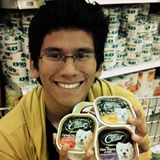
\includegraphics[width=0.3\textwidth]{Manuel}
    \caption{Foto de Manuel}
\end{figure}

Soy estudiante del sexto semestre y fundador de Sabrosoftware. Previamente trabajé con la compañía *insertar como se llamaba la compañía en donde trabajaba el Manuel* en donde nos enfocabamos al diseño y mantenimiento de páginas web.

Me gradué del bachillerato con especialidad técnica en Informática (2008 - 2011) lo cual me brindó un amplio panoráma de habilidades técnicas en el área de computación.

He participado en trabajos escritos en C++, Python, HTML y CSS. Fuí líder del primer proyecto de Sabrosoftware.

Mi meta es obtener experiencia en varias áreas de las Ciencias de la Computación, mejorar mis habilidades de programación y mejorar en el diseño de software.

\subsection{Flujo y relaciones de trabajo}

\begin{itemize}
\item \textbf{Líder del Proyecto:} Eduardo Acuña Yeomans
\item \textbf{Encargado de la Interfaz de Usuario:} Daniel Contreras Mejía
\item \textbf{Encargado del Diseño Algorítmico:} Francisco Manuel Valle Ruiz
\item \textbf{Encargado de la Documentación:} Eduardo Acuña Yeomans
\item \textbf{Encargado de Pruebas:} Francisco Manuel Valle Ruiz
\item \textbf{Encargado de Mantenimiento Técnico:} Daniel Contreras Mejía 
\end{itemize}

\begin{figure}[h!]
  \centering
    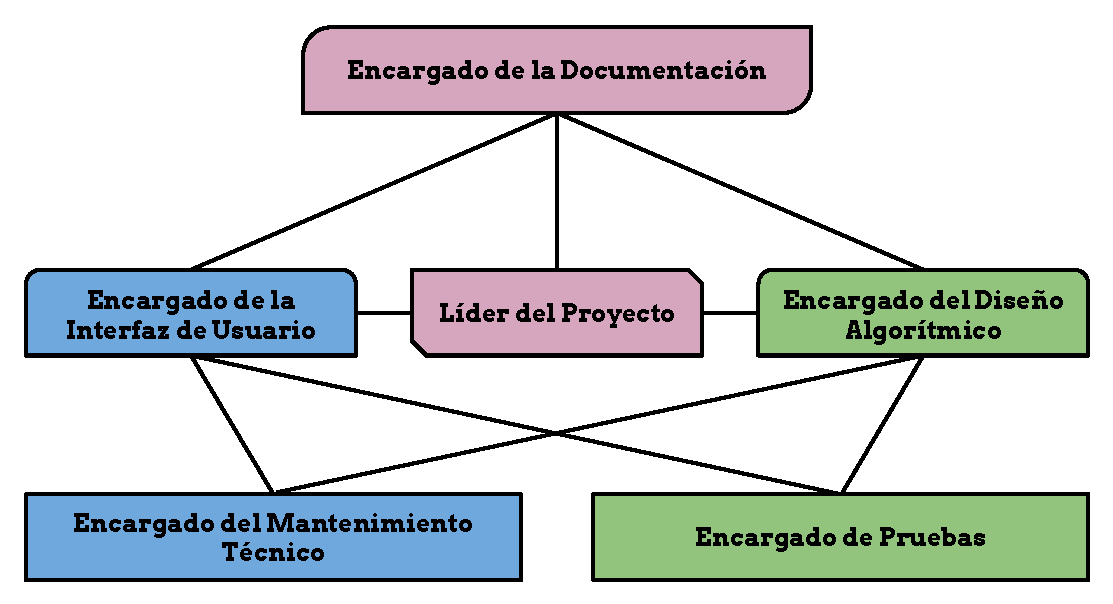
\includegraphics[width=0.9\textwidth]{Organigrama}
    \caption{Organigrama del equipo}
\end{figure}

El flujo de comunicación y trabajo se basa en desarrollo de documentos y códigos en plataformas colaborativas como Google Docs y GitHub, así como el uso de una lista de correos.

%%%
\section{Ámbito y Descomposición del software}
\subsection{Descripción del proyecto}
El problema planteado por el profesor Adrián es el de envío y recepción de oficios por parte de profesores y administrativos de la Universidad de Sonora. Nos mostró que la mayoría de los oficios que se redactan tienen practicamente el mismo formato y que el procedimiento de recepción es el de mandar el oficio al destinatario y que al llegar a la oficina correspondiente el oficio sea sellado de \emph{recibido}.

Se plantea desarrollar un sistema que emule este procedimiento. Las ideas que se mencionaron en clase fueron de generar documentos en formato PDF y manejar una especie de bandeja virtual para clasificar los documentos como recibidos o no recibidos, así como simplificar el proceso de darle formato a los oficios; se entendió que esta parte del sistema funcionara como el ``visto'' del facebook.

\subsection{Ámbito del proyecto}

Lo que se va a desarrollar en este proyecto es una pieza de software que pueda emular el proceso de entrega y recepción de oficios entre miembros de la Universidad de Sonora. En un primer prototipo se diseñará una versión simplificada del proceso y la implementación servirá como base para una futura evolución de el software.

Los oficios en cuestión son documentos con un formato determinado que un empleado redacta para imprimirlo y mandarlo a algún otro empleado u oficina de la Universidad, cuando este documento es recibido por el destinatario es sellado de recibido para tener como constancia que la comunicación se efectuó de manera oficial.

El software permitirá redactar y mandar oficios entre usuarios, manteniendo un control sobre cuándo se recibe el documento.

\subsection{Descomposición del proyecto}

Se opta por desarrollar una aplicación web para la implementación de este sistema. La ventaja es tanto para el usuario como para los desarrolladores ya que no será necesario descargar un programa para utilizar el sistema y los desarrolladores tendrán un control sobre toda la información debido a que será alojada en un servidor web.

Lograremos el cometido establecido separando el software en distintos módulos que interconectaremos para completar el funcionamiento efectivo del programa.

\begin{itemize}
\item Interfaz gráfica
\item Captura y validación de entradas
\item Generación de oficios
\item Control de entrega y recepción de oficios
\end{itemize}

Para simplificar la implementación de el proyecto, tendremos una base de usuarios preestablecida y un formato de oficios por defecto. Este prototipo se enfocará en la generación de oficios y el control de \emph{recibidos} y \emph{pendientes de revisar}.

\subsubsection{Módulo: Interfaz gráfica}
La interfaz gráfica será implementada sobre una página web, se separa en dos partes, descritas a continuación.

La primer parte es una bandeja de oficios en donde se podrán ver los oficios mandados y recibidos.

La segunda parte es una ventana de redacción de oficios, la cual tendrá los campos básicos de una ventana de envío de correo electrónico, con la posibilidad de previsualizar el documento antes de mandarlo y de elegir una plantilla para definir el formato del oficio. El programa tendrá una sola plantilla, pero es importante implementar el sistema con esta característica para futuro desarrollo.

\subsubsection{Módulo: Captura y validación de entradas}
La interfaz le va a permitir al usuario ingresar destinatarios, plantilla y el contenido del oficio. De estas entradas, la que se tiene que validar es la de los destinatarios, ya que se tienen que escribir usuarios que el sistema conozca. La validación de los destinatarios ocurrirá cuando el usuario intente previsualizar el documento o mande el oficio a los destinatarios. Esta validación consta en determinar si el campo de destinatarios tiene contenido y después determinar si los usuarios ingresados son válidos, es decir, si están registrados en el sistema.

\subsubsection{Módulo: Generación de oficios}
La generación de oficios entra en acción después de validar las entradas de la interfaz. Consiste en identificar cuatro elementos:
\begin{itemize}
\item La información del usuario que envía el oficio
\item La información de los destinatarios
\item El contenido del oficio
\item La plantilla de formato
\end{itemize}

La \emph{plantilla de formato} va a determinar cómo se acomodará la \emph{información de los usuarios} involucrados en el oficio y \emph{el contenido} redactado por el emisor. Al generar el documento con el formato deseado, se tendrá un archivo listo para ser enviado.

\subsubsection{Módulo: Control de entrega y recepción de oficios}
Ya teniendo identificados los usuarios involucrados en el envío del oficio y el archivo del documento, se realiza una entrega, notificando a los destinatarios que un oficio nuevo ha llegado a su bandeja.

Cuando los usuarios abran el documento, se notificará al usuario que mandó el oficio que el documento se recibió.

%%%
\section{Planificación}

\subsection{Análisis y selección de modelo}
Se utiliza el modelo por \emph{prototipos} ya que el cliente solo planteó una idea general del programa y será útil para los desarrolladores ir dejando los detalles sutiles para el final (debido a la poca experiencia que se tiene con este tipo de proyectos).

\subsection{Lista de actividades}

\begin{enumerate}
\item[1] \textbf{Analizar el problema:}
  \begin{enumerate}
  \item[1.1] Reunión con el cliente.
  \item[1.2] Aplicar un cuestionario de espectativas.
  \item[1.3] Determinar los puntos clave del sistema.
  \end{enumerate}
\item[2] \textbf{Diseñar el primer prototipo:}
  \begin{enumerate}
  \item[2.1] Determinar el cuerpo de conocimiento requerido y establecer las técnicas o métodos que el equipo debe aprender.
  \item[2.2] Establecer la interacción entre los diferentes componentes del software.
  \item[2.3] Analizar la manera en como el usuario interaccionará con el sistema.
  \item[2.4] Diseñar la interfaz de usuario.
  \item[2.5] Elegir o diseñar los algoritmos de generación de formato.
  \item[2.6] Elegir o diseñar los algoritmos de generación de archivos PDF.
  \item[2.7] Implementar el sistema.
  \end{enumerate}
  
  \item[3] \textbf{Pruebas al prototipo:}
    \begin{enumerate}
    \item[3.1] Probar el software con usuarios ficticios.
    \item[3.2] Probar el software con entradas usuales.
    \item[3.3] Probar el software con entradas erráticas.
    \end{enumerate}
    
  \item[4] \textbf{Correcciones:}
    \begin{enumerate}
    \item[4.1] Corregir validación de datos.
    \item[4.2] Corregir algoritmos de transformación.
    \item[4.3] Corregir interfaz de usuario.
    \end{enumerate}
    
  \item[5] \textbf{Documentación:}
    \begin{enumerate}
    \item[5.1] Documentación de usuario.
    \item[5.2] Documentación de desarrolladores.
    \item[5.3] Informe para el cliente.
    \end{enumerate}

  \item[6] \textbf{Reunión con el cliente:}
    \begin{enumerate}
    \item[6.1] Presentación del prototipo.
    \item[6.2] Anotación de cambios o mejoras.
    \end{enumerate}
\end{enumerate}

\subsection{Red de tareas}
En la \emph{Figura 2} se aprecia la dependencia de las actividades.
\begin{figure}[h!]
  \centering
  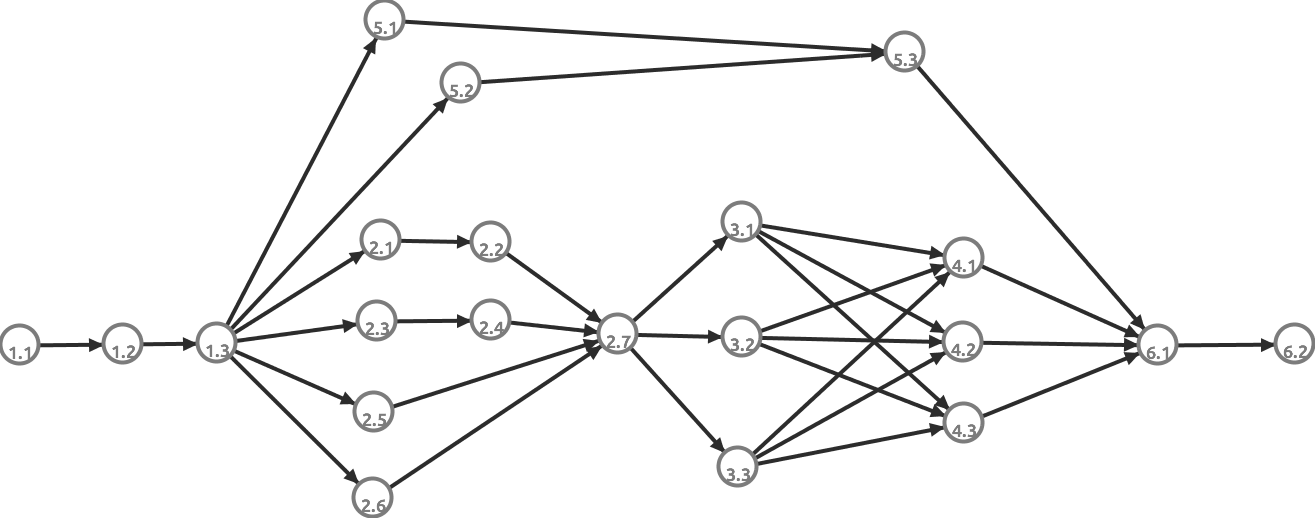
\includegraphics[width=1\textwidth]{RedTareas}
  \caption{Dependencia de tareas}
\end{figure}

\subsection{Carga de trabajo}

A continuación se presentan las actividades asignadas a cada integrante de Sabrosoftware.

\begin{itemize}
\item \textbf{Acuña Yeomans Eduardo:} 1.1, 1.2, 1.3, 2.7, 5.1, 5.2, 5.3, 6.1, 6.2.
\item \textbf{Contreras Mejía Daniel:} 1.1, 2.1, 2.2, 2.3, 2.4, 2.7, 4.1, 4.3, 6.1.
\item \textbf{Valle Ruiz Francisco Manuel:} 1.1, 2.5, 2.6, 2.7, 3.1, 3.2, 3.3, 4.2, 6.1.
\end{itemize}

\subsection{Diagrama de Gantt}
En la \emph{Figura 3} se aprecia la distribución corregida de las actividades.
\begin{figure}[h!]
  \centering
  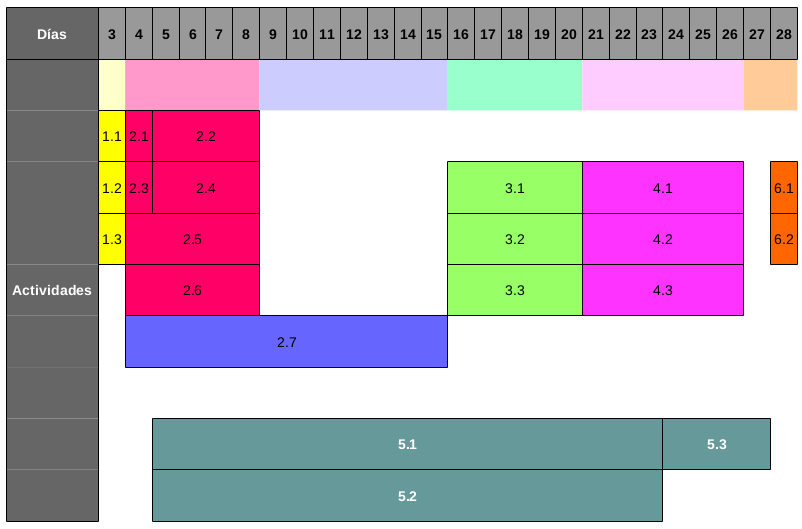
\includegraphics[width=.80\textwidth]{Gantt.png}
  \caption{Diagrama de Gantt}
\end{figure}

%%%
\section{Análisis de Riesgo}

\subsection{Posibles problemas}
\begin{itemize}
\item Pérdida de datos
\item Ausencia de integrantes del equipo
\item Imposibilidad de comunicación por incompatibilidad de horario
\end{itemize}

\subsection{Plan de contención}
Para evitar los potenciales riesgos que se pueden presentar a lo largo del desarrollo del proyecto, se opta por trabajar de manera defensiva y prevenir los sucesos con mas probabilidad de ocurrencia.

\begin{itemize}
\item Toda la documentación y código del proyecto será trabajada sobre un repositorio en Github, en donde se podrá observar y obtener métricas de cómo evoluciona el trabajo. De esta manera, cualquier problema de pérdida de datos, será minimizado por el respaldo permanente de cada una de las versiones (con la posibilidad de rastrear cada cambio).
\item Si por algún motivo un integrante del equipo no puede realizar la labor asignada, el líder del proyecto se hará cargo de dicha labor de manera personal.
\item La comunicación se realizará obligatoriamente vía correo electrónico y presencial de manera opcional.
\end{itemize}

%%%
\section{Presupuestación}
La presupuestación del proyecto se realizó de dos maneras: por Líneas de Código (LDC) y Puntos de Función (PF), las cuales se describen a continuación.

\subsection{En base a Líneas de Código}
Se retoma la división modular de la sección de la \emph{Descomposición} para aproximar las líneas de código estimadas.

\begin{itemize}
\item Interfaz gráfica \textbf{LDC: 100}
\item Captura y validación de entradas \textbf{LDC: 50}
\item Generación de oficios \textbf{LDC: 200}
\item Control de entrega y recepción de oficios \textbf{LDC: 100}
\end{itemize}

Esta asignación numérica resulta con un total de \textbf{450} líneas de código. Asumiendo que el sueldo mensual por persona es de $\$5,000^{00}$ y que la cantidad de líneas de código al mes por persona son 150. Determinamos que el precio por línea de código es de $\$33^{00}$. Por lo tanto, el precio estimado del proyecto es de $450 * \$33^{00} = \$14,850^{00}$ y el tiempo estimado del proyecto es de $450/(150*3)=1$ mes.

\subsection{En base a Puntos de Función}
Al obtener los \emph{puntos de función} totales del proyecto se establecerán una serie de medidas para poder realizar la estimación del presupuesto.

\begin{enumerate}
\item \textbf{Entradas externas}
  \begin{itemize}
  \item Datos del oficio a mandar
  \item Datos del usuario
  \end{itemize}
\item \textbf{Salidas externas}
  \begin{itemize}
  \item Interfaz gráfica
  \item Mensajes de error
  \item Visualización de documentos
  \end{itemize}
\item \textbf{Consultas externas}
\item \textbf{Archivos lógicos internos}
  \begin{itemize}
    \item Estructura del formato
    \item Estructura del contenido del oficio
    \item Usuarios
  \end{itemize}
\item \textbf{Archivos de interfaz externas}
  \begin{itemize}
  \item Datos de los usuarios
  \end{itemize}
\end{enumerate}

Ya que se identifica la cantidad de componentes por categoría, se llena la siguiente tabla:

\begin{figure}[h!]
  \begin{tabular}{ l c c c c c c c }
    Dominio & Conteo &  & S & P & C & & resultado \\
    Entradas externas & 2 & $\times$ & 3 & 4 & 6 & $=$ & 8\\
    Salidas externas & 3 & $\times$ & 4 & 5 & 7 & $=$ & 15\\
    Consultas externas & 0 & $\times$ & 3 & 4 & 6 & $=$ & 0\\
    Archivos lógicos internos & 3 & $\times$ & 7 & 10 & 15 & $=$ & 30\\
    Archivos de interfaz externas & 1 & $\times$ & 5 & 7 & 10 & $=$ & 7\\
    Total & & & & & & $=$ & 60 \\ 
  \end{tabular}
  \caption{Tabla para la ponderación de PF}
\end{figure}

\textbf{Nota:} Ya que no se ha realizado un proyecto como este, se estimaron como tareas ``promedio'' y es así como se ponderan estos dominios para el conteo de los puntos de función.

El siguiente paso es establecer los factores de ajuste, Pressman determina que a estas 14 preguntas se les tiene que asignar un número entre 0 (no importante) y 5 (escencial).

\begin{enumerate}
\item ¿El sistema requiere respaldo y recuperación confiable? \textbf{2}
\item ¿Comunicación de datos especializada es requerida para la transferencia de información? \textbf{0}
\item ¿Hay funciones de procesamiento distribuido? \textbf{0}
\item ¿Es el rendimiento crítico? \textbf{1}
\item ¿El sistema será ejecutado en ambientes altamente utilizados? \textbf{2}
\item ¿Requiere entradas de datos en línea? \textbf{5}
\item ¿Se requieren múltiples pantallas u operaciones para la transacción de información en línea? \textbf{1}
\item ¿Los archivos lógicos internos son actualizados en línea? \textbf{3}
\item ¿Hace uso de archivos de entrada/salida complejos? \textbf{2}
\item ¿Realiza procesamiento interno complejo? \textbf{2}
\item ¿El código está diseñado para ser reutilizado? \textbf{2}
\item ¿Se incluye instalación y conversión en el diseño? \textbf{0}
\item ¿El sistema está diseñado para múltiples instalaciones en diferentes organizaciones? \textbf{0}
\item ¿La aplicación está diseñada para facilitar cambios y fácil uso por el usuario? \textbf{0}
\end{enumerate}

Dada esta valoración el \emph{total de factores de ajuste} es \textbf{20}; para obtener el valor de \emph{puntos de función (PF)} se usa la fórmula:
\begin{align*}
  PF &= ConteoPonderado \times [0.65+0.01 \times ConteoAjuste] \\
  PF &= 60 \times [0.65 + 0.01 \times 20] \\
  PF &= 60 \times [0.65 + 0.2] \\
  PF &= 60 \times 0.85 \\
  PF &= 51
\end{align*}

Decidimos que no se estimará el presupuesto ni el tiempo de desarrollo con Puntos de Función ya que no tenemos datos históricos con que trabajar. Sin embargo, se calcula este valor para realizar la estimación ya terminado el primer prototipo.

\end{document}
